\subsection{View Elimination}
\label{ssec:arith_view}

The imperative control flow is generated from compiling declarative smart contracts, ensuring the maintenance of all relations defined by the Datalog rules. The compilation process is basically divided into two distinct phases. In the first phase, it identifies the set of update operators that might occur during the execution of the smart contract, including the insertion, deletion, or update of relational tuples. In the second phase, once the updates are identified, they trigger the corresponding contract rules for updating. Note that inference rules are triggered whenever any of their body relations are updated, whereas transaction rules are only triggered by their declared events. For each rule, the resulting imperative maintenance procedures typically involve looking up relational tuples within the rule body, validating the rule constraints, and generating updates for the rule head. Notably, any changes to the updated rule head can also lead to updates in subsequent associated rules.

Given this imperative control flow, we introduce arithmetic optimization techniques to eliminate intermediate views and variables.

% \noindent \textbf{Arithmetic simplification.}
% \label{ssec:arith_view}
% Previous research on incremental view maintenance,
% such as Differential Dataflow~\cite{mcsherry2013differential} and
% Timely Dataflow~\cite{murray2013naiad}, has predominantly focused on
% database operators like joins and aggregations, handling changes
% such as tuple insertions, deletions, and updates.
% While these techniques have proven effective in optimizing the execution
% flow of declarative smart contracts (e.g., DeCon~\cite{chen2022declarative}),
% the inclusion of arithmetic operators in DeCon introduces new opportunities
% for further optimizations.

Take the rule in Figure~\ref{fig-example} Line 14 as an instance. It defines the balance of an address {\sf \lstinline{p}} as the difference between the sum of its incoming transfers {\sf \lstinline{i}} and the sum of its outgoing transfers {\sf \lstinline{o}}. Let us assume a new transfer {\sf \lstinline{transfer(p,q,10)}} is committed, leading to an increment of {\sf \lstinline{totalOut[p]}} by $10$. If we were to interpret this rule as a regular join rule, as depicted in the bottom-left portion of Figure~\ref{fig:arith-opt}, the incremental maintenance procedure would involve retrieving the sum of incoming transfers of {\sf \lstinline{p}}, storing it in local memory as {\sf \lstinline{i}}, and then computing the new balance by subtracting {\sf \lstinline{o}} from {\sf \lstinline{i}}. However, upon analyzing the arithmetic operator, we can deduce that the update amount is $-10$. This insight gives rise to a simpler update approach, as demonstrated in the bottom-right section of Figure~\ref{fig:arith-opt}: we can directly decrement {\sf \lstinline{balanceOf[p]}} by $10$, eliminating the need for storage retrieval and local computation.

\begin{figure}[t]
    \centering
    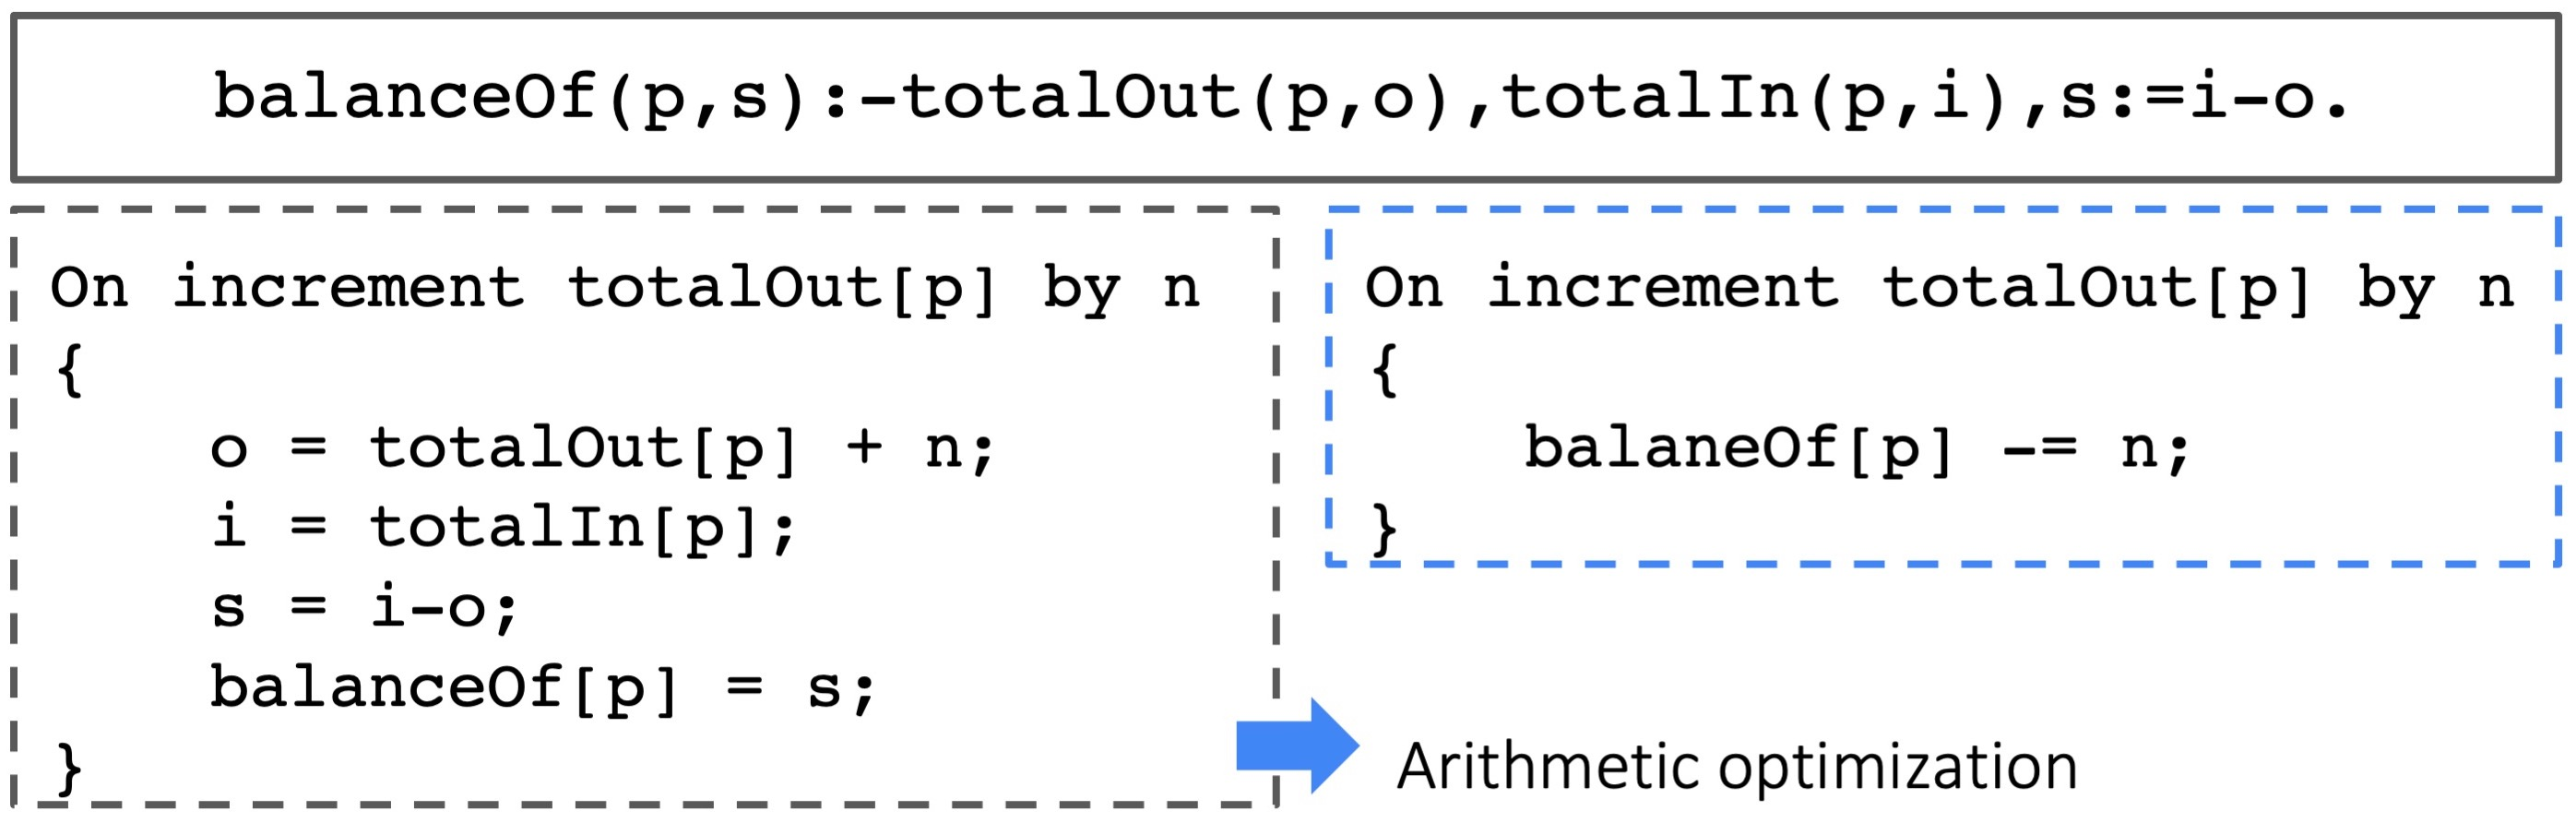
\includegraphics[width=0.45\textwidth]{figures/arithmetic-optimization.jpg}
    \caption{Incremental update without (left) and with (right)
        arithmetic optimization.}
    \label{fig:arith-opt}
\vspace{-1.5em}
\end{figure}

Essentially, we aim to identify a differentiable fragment within the update procedure that enables us to update its dependent head relations solely based on the amount of change, without relying on the specific value itself. In the above example, {\sf \lstinline{totalOut[p]}} is such a differentiable fragment. Since this update is agnostic to the concrete value of {\sf ``totalOut''}, we can save unnecessary storage reads and computation costs when updating {\sf ``balance''}. Meanwhile, since there are no other places that query the {\sf ``totalOut''} relation, we can directly identify {\sf ``totalOut''} as a transient relation and eliminate it from the imperative control flow, which further saves the costs for recomputing and rewriting {\sf ``totalOut''} in storage. Similarly, {\sf ``totalIn''} can also be eliminated. Overall, the idea of differentiable fragments here is general and can be extended to addition, subtraction, aggregation, count, and even multiplication.


\proto identifies such differentiable fragments by checking all update procedures to all rules, and eliminates both the read and write operations to these transient relations. Through this pass, \proto eliminates relations that are not accessed by any update procedure from the imperative control flow.